\section{DSC and TGA techniques for 3D-printing of polymers}

A \gls{tga} measurement makes it possible to determine the temperature in which the polymer is stable, i.e. above some temperatures the polymer starts to degradate(fig. \ref{fig:TGA_DSC}). 
This information is important when 3D-printing techniques are used in which the polymer is subjected to higher temperatures. Furthermore, when a \gls{dsc} test would be performed it is important 
to know the bounds on the temperature. 

\gls{dsc} is usefull for 3D-printing since it gives information on how a sample physically and chemically changes upon endothermal or exothermal processes or changes in heat capacity. On figurre \ref{fig:TGA_DSC} the \gls{dsc} curve displays the differential heat flow in function of the temperature. 
The peaks indicate that the material undergoes a transition. This information is crucial for picking the right temperature in which the 3D-printing processes needs to take place\citec{JASON2022}.

\begin{figure}[ht]
    \centering
    \begin{subfigure}[b]{0.4\textwidth}
        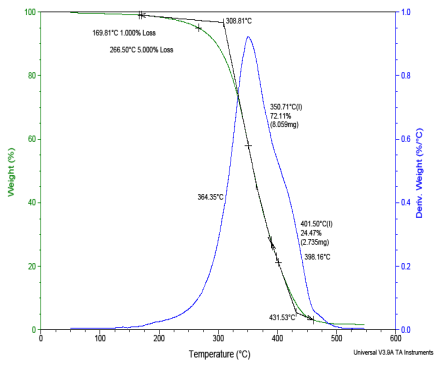
\includegraphics[width=\textwidth]{TGA.png}
    \end{subfigure}
    \begin{subfigure} [b]{0.5\textwidth}
        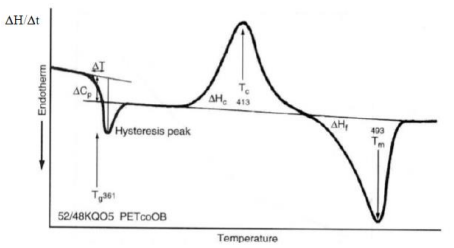
\includegraphics[width=\textwidth]{DSC.png}
    \end{subfigure}
    \caption{Typical TGA curve (left) and typical DSC curve (right)}
    \label{fig:TGA_DSC}
\end{figure}